\chapter{Использование семантических технологий и распределенных систем в образовательном процессе} \label{chapt1}


\section{Характеристики и задачи распределенных систем} \label{sect1_1}

Распределенная система — это набор независимых компьютеров, представляющийся их пользователям единой объединенной системой \cite{tanenboum2003raspr}.

Одним из примеров  распределенной системы является сеть WWW (World Wide Web). Данная система предоставляет простую, целостную и единообразную модель распределенных документов. Чтобы увидеть документ, пользователю достаточно активизировать ссылку. После этого документ появляется на экране. 

Одно из главных требований к распределенной системе это ее единство в представлении пользователя. Применение распределенных систем стало актуальным при значительном увеличении скорости передачи данных между независимыми компьютерами и возникновении необходимости проведения трудоемких вычислительных задач. Распределенные системы в первую очередь заменяют дорогостоящие суперкомпьютеры \cite{shokin1998raspr}. Главным преимуществом системы из независимых компьютеров является возможность ее масштабирования путем добавления или удаления из системы новых машин. Такие системы позволяют производить трудоемкие вычисления, объединять удаленные базы знаний в единое облако и предоставлять необходимые услуги пользователям, скрывая от них свое реальное местоположение \cite{wang2010distributed}.

Распределенная система обладает рядом характеристик. Первая из таких характеристик состоит в том, что от пользователей скрыты различия между компьютерами и способы связи между ними. То же самое относится и к внешней организации распределенных систем. Другой важной характеристикой распределенных систем является способ, при помощи которого пользователи и приложения единообразно работают в распределенных системах, независимо от того, где и когда происходит их взаимодействие. Распределенные системы должны также относительно легко поддаваться расширению, или масштабированию \cite{coulouris2005distributed}. Эта характеристика является прямым следствием наличия независимых компьютеров, но в то же время не указывает, каким образом эти компьютеры на самом деле объединяются в единую систему. Распределенные системы обычно существуют постоянно, однако некоторые их части могут временно выходить из строя. Пользователи и приложения не должны уведомляться о том, что эти части заменены или починены или что добавлены новые части для поддержки дополнительных пользователей или приложений.

Основными задачами распределенных систем являются:

\begin{itemize}
\item соединение пользователей с ресурсами. Распределенная система должна облегчить пользователям доступ к удаленным ресурсам и обеспечить их совместное использование, регулируя этот процесс \cite{ghosh2014distributed}. Ресурсы могут быть виртуальными, однако традиционно они включают в себя принтеры, компьютеры, устройства хранения данных, файлы и данные. Web-страницы и сети также входят в этот список. 
\item скрытие факта, что процессы и ресурсы физически распределены по множеству компьютеров. Распределенные системы, которые представляются пользователям и приложениям в виде единой компьютерной системы, называются прозрачными.
\item предоставление служб со стандартным синтаксисом и семантикой. В распределенных системах службы обычно определяются через интерфейсы, которые часто описываются при помощи языка определения интерфейсов.
\item обеспечение масштабируемости системы. Масштабируемость системы может измеряться по трем различным показателям. Во-первых, система может быть масштабируемой по отношению к ее размеру, что означает легкость подключения к ней дополнительных пользователей и ресурсов. Во-вторых, система может масштабироваться географически, то есть пользователи и ресурсы могут быть разнесены в пространстве. В-третьих система может быть масштабируемой в административном смысле, то есть быть проста в управлении при работе во множестве административно независимых организаций. Система, обладающая масштабируемостью по одному или нескольким из этих параметров, при масштабировании часто дает потерю производительности.
\end{itemize}

Сама распределенная система является лишь фундаментом для реализации более сложных сетевых и системных взаимодействий. Внутри распределенной системы могут быть описаны механизмы обмена данными, поддержания работоспособности системы \cite{jalote1994fault}, распределения нагрузки на систему \cite{shirazi1995scheduling} и безопасности передачи данных внутри системы \cite{chen2011parallel}. 

Примером реализации системы основанной на принципах и механизмах распределенной системы является система электронного обучения \cite{masud2012learning}. Система электронного обучения решает с помощью механизмов распределенной системы задачи по масштабируемости системы и представления системы в виде единой службы \cite{masud2012novel}. 


\section{Классификация систем дистанционного обучения и их развитие в России и за рубежом} \label{sect1_2}

Система электронного обучения - это система управления учебной деятельностью. Система электронного обучения позволяет разрабатывать, управлять и распространять учебные онлайн-материалы с обеспечением совместного доступа. Данный вид систем предназначен для проведения удаленного дистанционного образовательного процесса включающего в себя процесс получения знаний и процесс проверки знаний пользователя \cite{keegan1996foundations}.

Существует несколько вариантов использования технологий электронного обучения:

\begin{itemize}
\item в качестве дополнительной поддержки основного курса обучения (здесь технологиям электронного обучения отводится вспомогательная роль),
\item в качестве основы для самообразования (в этом случае учащиеся самостоятельно приобретают и осваивают готовые электронные образовательные продукты, например - мультимедиа курсы),
\item в качестве основной образовательной технологии \cite{mojaeva2000edu}. В этом случае создается постоянная группа учащихся в периферийном центре, которая работает под руководством и под контролем педагога или координатора. Он контролирует ход учебного процесса, своевременное выполнение заданий учащимися, консультирует, помогает учащимся в процессе освоения курса.
\end{itemize}

На данный момент существует два вида электронного обучения: 

\begin{itemize}
\item асинхронное электронное обучение, которое предусматривает, что ученик сам определяет темп своего обучения. При этом обучающийся имеет выбор между различными носителями информации, ученик может выполнять задания в соответствии с аудиторной программой или планом, а затем передавать готовую работу преподавателю для оценки.
\item синхронное электронное обучение \cite{azinadistance}. Данный вид предусматривает общение учеников и преподавателей в реальном времени через виртуальные аудитории. 
\end{itemize}

Историю развития электронного обучения можно разделить на несколько поколений:

\begin{itemize}
\item 1-ое поколение. Технические средства, характеризующиеся отсутствием интерактивности (радио или аудио кассеты, учебники, посланные студентам с минимальным общением по телефону).
\item 2-ое поколение. Асинхронно интерактивные курсы, характеризующиеся трансляциями (телевидение или радио) с призывом к интерактивности (в течение или после) либо по телефону, либо по электронной почте.
\item 3-е поколение. Характеризуется использованием веб-страниц с программой обучения, другими статическими материалами и чат-сессиями, обеспечивающими интерактивное общение.
\item 4-ое поколение. Интерактивность в реальном времени с программным обеспечением, видеокамерами, объединенной системой управления \cite{rad2005create}.
\end{itemize}

Сегодня появляется необходимость и возможность говорить о медиа-обучении, то есть о массовом медиа-образовании\cite{dabbagh2012personal}. Его предпосылкой является развитие новых технологий, прежде всего – компьютерных. Одним из плацдармов, на котором можно эффективно и целенаправленно развернуть формирование и информационной, и медиа-культуры, являются дистанционные технологии образования средствами Интернета. Они могут послужить противовесом деструктивному воздействию идеологии социального конструкционизма в практике медиа \cite{kalmikov2009learning}.

Задачи и принципы медиа-образования пока не входят непосредственно в содержание образовательных программ. Иными словами, можно констатировать, что дистанционное образование является до сих пор неиспользованным ресурсом формирования информационной культуры. 

Системы электронного обучения в зарубежных странах имеют развитую инфраструктуру и широкую пользовательскую аудиторию. Так, например, Открытый университет Великобритании (The Open University) имеет 305 региональных центров в Великобритании и 42 в других странах. Испанский национальный университет дистанционного образования имеет 53 региональных центра в Испании и Латинской Америке. Канадский открытый университет имеет 4 региональных центра. Ферн Университет Германии имеет 60 региональных центров в Германии, Австрии, Голландии, Венгрии, Польше. Открытый университет Израиля располагает более чем 100 региональными центрами. Национальный технологический университет США использует для обучения более 300 площадок на базе 46 вузов США \cite{korneeva2007state}. 

В США интенсивно развивается предоставление интерактивных онлайн-курсов. К 2009 году более 5,6 миллионов студентов приняло участие в прохождении хотя бы одного онлайн-курса. Около 30\% процентов студентов получающих высшее образование участвуют в электронном обучении. Использование систем электронного обучения привело к росту количества студентов, получающих высшее образование на два процента \cite{allen2010class}.

В зарубежных странах интенсивно развивается предоставление учебных материалов в формате массовы открытых онлайн-курсов MOOC (Massive open online courses) \cite{pappano2012year}. MOOC система предоставляет пользователям набор обучающих курсов с массовым интерактивным участием c применением технологий электронного обучения и открытым доступом через Интернет \cite{mcauley2010mooc}. MOOC системы дают возможность использовать интерактивные форумы пользователей, которые помогают создавать и поддерживать сообщества студентов, преподавателей и ассистентов.

Крупнейшей MOOC системой является портал Coursera. Портал сотрудничает с университетами, которые публикуют и ведут в системе курсы по различным отраслям знаний. Слушатели проходят курсы, общаются с сокурсниками, сдают тесты и экзамены непосредственно в системе. Портал использует более 13 миллионов студентов. Coursera предоставляет более тысячи бесплатных онлайн-курсов от более чем 100 ведущих мировых вузов. На портале представлены курсы по физике, инженерным дисциплинам, гуманитарным наукам и искусству, медицине, биологии, математике, информатике, экономике и бизнесу. Продолжительность курсов примерно от шести до десяти недель, с 1—2 часами видеолекций в неделю, курсы содержат задания, еженедельные упражнения и иногда заключительный проект или экзамен \cite{knox2012mooc}.

Другой крупной MOOC системой явялется платформа edX. edX разработана Гарвардским университетом и Массачусетским технологическим институтом и распространяется в формате открытого программного кода. Платформа позволяет любой организации на базе своих курсов развернуть систему MOOC \cite{breslow2013studying}. На платформе развернуто более 500 онлайн-курсов. Плаформой edX пользуется более 2,5 миллионов студентов. 

Также бесплатные массовые открытые курсы предоставляет проект Udacity \cite{salmon2012udacity}. Udacity проект, возникший на базе программы по информатике Стэнфордского университета. Проект предоставляет видеолекции на английском языке с субтитрами в сочетании со встроенными тестами и последующими домашними работами. Каждая лекция включает в себя встроенный тест, чтобы помочь студентам понять предлагаемые концепции и идеи. Проект предоставляет более 80 курсов для более 1,5 миллионов студентов.

Системы MOOC получили развитие в различных зарубежных странах. Проект Iversity разработан в Германии и используется более чем 300 тысячами студентов. Проект Open Univercity основан на базе открытого университета Великобритании. Портал Crypt4you предоставляет MOOC курсы в Испании. OpenupEd — проект MOOC системы образовательных структур Евросоюза. Проект EduKart предоставляет MOOC курсы в Индии.

Привлекательность MOOC систем заключается в их бесплатности для вузов, государства, обучающихся, которая является следствием того, что:

\begin{itemize}
\item нет необходимости создавать свои учебники и учебно-методические материалы;
\item не нужно финансировать образовательный процесс и научные исследования в вузах;
\item не нужны сами вузы и, как следствие, научно-педагогические работники;
\item получать высшее образование можно бесплатно в любое удобное время \cite{kollesnicov2014aprch}.
\end{itemize}

В России системы электронного обучения имеют менее развитую инфраструктуру и находятся на этапе становления. Проблема дистанционного образования представляется особенно важной для России с ее огромной территорией, неравномерной плотностью населения и размещением вузовских центров.

Актуальность развития дистанционного образования на территории Российской Федерации обуславливается следующими тенденциями:

\begin{itemize}
\item Россия испытывает на себе влияние процессов глобализации, информатизации образовательной среды. Как результат - подписание Болонского соглашения и следующие за ним демократизация, открытость образования, внедрение дистанционных технологий обучения.
\item с начала 90-х годов в России наблюдается недостаток востребованных рынком специалистов. Изменения в экономической сфере побуждают вузы к открытию новых специальностей, стимулируют развитие негосударственного сектора образования, более мобильного и адаптированного к запросам потребителя, в том числе по формам и технологиям обучения.
\item нарастает конкуренция вузов за потребителя, вызванная, с одной стороны, появлением наряду с государственными вузами негосударственных, с другой стороны, ухудшением демографической ситуации.
\end{itemize}

Для улучшения качества электронного обучения необходимо восстановить полную структуру системы обучения, добавив в нее повсеместно отсутствующие в России отделы преподавания и разработки учебников. Крайне важно привлечь в указанные отделы наиболее опытных и квалифицированных преподавателей, которые бы занимались только своими прямыми обязанностями \cite{levin2005system}. 

Одним из крупнейших открытых ресурсов, предоставляющих онлайн-курсы, в России является Национальный Открытый Университет <<ИНТУИТ>>. <<ИНТУИТ>> предоставляет услуги по нескольким образовательным программам, многие из которых касаются информационных технологий. Так же <<ИНТУИТ>> функционирует как издательство, выпуская учебную литературу по курсам. В <<ИНТУИТ>> можно пройти более 820 курсов по различным областям информатики — в том числе, изучить различные языки программирования и разметки, численные методы и параллельные вычисления. Кроме того, портал предоставляет курсы по физике, математике, экономике и философии. Отдельные образовательные программы ведут такие компании как Microsoft и Intel. На <<ИНТУИТ>> проходит обучение более 16 тысяч студентов.

Другим крупным открытым образовательным ресурсом в России является проект <<Лекториум>>. Проект <<Лекториум>> – медиатека, в которой публикуются лучшие видеолекции вузов и известных лекториев России. <<Лекториум>> записывает лекции различных образовательных площадок, среди которых Computer Science Center, Математическая лаборатория имени П.Л. Чебышева, Музей Анны Ахматовой и другие. Проект предоставляет слушателям курсы в формате MOOC \cite{nilova2014mooc}. В проекте размещено более 318 курсов и более чем 4 тысячи часов видеолекций. В <<Лекториум>> проходит обучение более 50 тысяч студентов. 

Достоинствами систем электронного обучения являются:

\begin{itemize}
\item технологичность - обучение с использованием современных программных и технических средств делает электронное обучение более эффективным; 
\item доступность и открытость обучения - возможность учиться удалено от места обучения, не покидая свой дом или офис; 
\item свобода и гибкость - появляются новые возможности для выбора курса обучения. Очень легко выбрать несколько курсов из разных университетов, из разных стран. 
\item индивидуальность систем электронного обучения. Электронное обучение является более гибким и носит более индивидуальный характер обучения. Обучающийся сам определяет темп обучения, может возвращаться по несколько раз к отдельным урокам, может пропускать отдельные разделы и т.д. 
\item внедрение электронного обучения уменьшает нервозность студентов при сдаче зачета или экзамена. 
\end{itemize}

Недостатками систем электронного обучения являются:

\begin{itemize}
\item отсутствие прямого очного общения между студентами и преподавателем;
\item необходимость в персональном компьютере и доступе в Интернет;
\item проблема аутентификации пользователя при проверке знаний;
\item контроль актуальности и качества учебных материалов; 
\item высокая трудоемкость разработки курсов электронного обучения. 
\end{itemize}

Инфраструктура системы электронного образования включает в себя центр ДО (ЦДО) базового образовательного учреждения и периферийные центры ДО (ПЦДО), связывающие их телекоммуникационные каналы и размещенные в центрах информационные ресурсы.

Построение распределенной образовательной среды позволяет снять ряд проблем, связанных с доступом к учебной информации. Создание локальных копий Web-ресурсов, их репликация и синхронизация позволяют обеспечить доступ средствами Интранет и значительно уменьшить Интернет-трафик.

Одним из недостатков в современных системах электронного обучения является ограниченные  возможности повторного использования учебных материалов. В целях упрощения интеграции сторонних учебных материалов в систему электронного обучения был разработан стандарт SCORM (Sharable Content Object Reference Model). SCORM cодержит требования к организации учебного материала и архитектуры системы электронного обучения \cite{parmar2012paper} \cite{qu2002towards}. Стандарт позволяет обеспечить совместимость компонентов и возможность их многократного использования. Учебный материал представлен отдельными небольшими блоками, которые могут включаться в разные учебные курсы и использоваться системой дистанционного обучения независимо от того, кем, где и с помощью каких средств они были созданы. SCORM основан на стандарте XML.

Недостатками стандарта SCORM являются:

\begin{itemize}
\item ограниченный выбор видов деятельности;
\item низкая безопасность;
\item ограничения в поддержке и редактировании материалов;
\item сложный формат представления данных;
\item ограничения по совместимостью с различными системами электронного обучения;
\item использование большого количества интернет-трафика и времени загрузки \cite{bohl2002sharable}.
\end{itemize}

Для решения озвученных проблем на основе стандарта SCORM был разработан новый стандарт Tin Can API. Новый стандарт разработан с использованием новейших технологий HTML5 и JavaScript и делает учебные объекты более интерактивными \cite{poltrack2012next}. Tin Can API не содержит недостатков стандарта SCORM. В Tin Can API произведена адаптация с мобильными устройствами, добавлены интерактивные симуляторы и игры. В стандарте улучшена безопасность и присутствует возможность отслеживания и аналитики активности пользователя \cite{regan2013training}. 

Одним из основных недостатков стандартов SCORM и Tin Can API является отсутсвие семантики в описании учебных материалов. Данный недостаток не позволяет, при использовании данных стандартов в системе электронного обучения, производить машинный вывод, гармонизацию и агрегацию данных используя данные с различных источников в различных форматах. Описание данных в стандартах ограничивается описанием учебных материалов, что затрудняет возможность интеграции и связывания учебных материалов с данными социальных сетей или баз знаний других предметных областей \cite{del2013learning}.   


Технологическая компонента системы электронного обучения позволяет предоставлять учебные материалы в не только в текстовых форматах, но и с использованием мультимедиа \cite{schlosser2009distance}. Данный формат представления информации позволяет пользователю системы лучше усваивать учебный материал \cite{moore2011distance}.

Согласно теории двойного кодирования информация воспринимается по одному из двух обычно независимых каналов \cite{monahova2013multi}. Один канал воспринимает устную информацию типа текста или аудио. Другой канал воспринимает невербальные изображения типа иллюстраций и звуков в окружающей среде. Информация может восприниматься через оба канала одновременно. Информация, переработанная таким образом, называется референциальной и имеет суммарный эффект на запоминание. Усваивание происходит лучше, когда информация воспринимается через два канала, чем через один канал. Референциальная обработка может производить этот суммарный эффект, потому, что обучающийся создает больше познавательных путей, по которым можно следовать, чтобы отыскать нужную информацию. Использование аудио с видео может задействовать множественные мозговые процессы, приводя к лучшему запоминанию.

Электронное обучение, индивидуализированное по своей сути, не должно вместе с тем исключать возможностей коммуникации не только с преподавателем, но и с другими учащимися, сотрудничества в процессе разного рода познавательной и творческой деятельности. Проблемы социализации оказываются весьма актуальны при электронном обучении \cite{hu2013revised}. 

Способами повышения качества систем электронного обучения и решения основных проблем при работе с ними являются: 

\begin{itemize}
\item стимулирование разработки качественных информационных ресурсов,
\item облегчение процесса публикации материалов, 
\item информирование образовательного сообщества о новых материалах,
\item привлечение авторитетных источников, 
\item механизмы рецензирования \cite{ivannicov2003common}.
\end{itemize}

Одним из перспективных способов повышения качества системы электронного обучения является использование в ней онтологий и семантических технологий.




\section{Онтологии, экспертные системы, базы знаний и семантические сети} \label{sect1_3}

Онтология - это система, состоящая из набора понятий и набора утверждений об этих понятиях, на основе которых можно строить классы, объекты, отношения, функции и теории. Онтология представляет собой некоторое описание взгляда на мир применительно к конкретной области интересов. Это описание состоит из терминов и правил использования этих терминов, ограничивающих их значения в рамках конкретной области. Иными словами онтология - это явное описание концептуализации. Концептуализация – это структура реальности, рассматриваемая
независимо от словаря предметной области и конкретной ситуации \cite{solov2006ontology}. 

Основными компонентами онтологии являются:

\begin{itemize}
\item классы или понятия,
\item отношения,
\item функции,
\item аксиомы,
\item примеры.
\end{itemize}

Существует два альтернативных подхода к созданию и исследованию онтологий. Первый (формальный) основан на логике (предикатов первого порядка, дескриптивной, модальной и т.п.). Второй (лингвистический) основан на изучении естественного языка (в частности,
семантики) и построении онтологий на больших текстовых массивах, так называемых корпусах

Web-онтология может включать описание классов, и их свойств, а также индивиды классов. Онтологии в состоянии сыграть критически важную роль в организации обработки знаний на базе Web, их совместного использования и обмена между приложениями. Онтологии в общем виде определяемые как совместно используемые формальные концептуализации конкретных предметных областей, дают общеее представление о темах, информацией по которым могут обмениваться люди и приложения \cite{suarez2012ontology}. 

Основными структурными элементами языка онтологий являются понятия класса, индивида и свойства. Класс - это простое название и совокупность свойств, которые описывают набор индивидов. Классы онтологии составляют таксономию — иерархию понятий по отношению вложения \cite{lapshin2010ontology}. Индивиды - это сущности, которые, если они удовлетворяют всем свойствам класса, являются его экземплярами. Индивиды могут представлять собой как физические объекты (люди, дома, планеты), так и абстрактные (числа, слова). Строго говоря, онтология может обойтись и без конкретных объектов. Однако, одной из главных целей онтологии является классификация таких объектов, поэтому они также включаются. Таким образом, классы должны соответствовать естественно образованным наборам вещей в рассматриваемой области, а индивиды должны соответствовать реальным объектам, которые могут быть сгруппированы в эти классы. Свойства позволяют нам утверждать общие факты об экземплярах классов и особые факты об индивидах \cite{shumski2010preobraz}. Свойства могут описывать простые данные или сложные объекты. Важная роль свойств заключается в том, чтобы определять отношения (зависимости) между объектами онтологии. Обычно отношением является свойство, значением которого является другой объект.

%%%%%%%%%%%%%%%%%%%%%%%%%%%%
% Можно еще полить воды если не хватит
%%%%%%%%%%%%%%%%%%%%%%%%%%%%%%%%%

Семантика — это наука, устанавливающая отношения между символами и объектами, которые они обозначают, то есть наука, определяющая смысл знаков. Применение семантики в информационных технологиях наиболее ярко отражено в разделе по разработке искусственного интеллекта. С помощью семантики разрабатываются различные экспертные системы.

Экспертная система, прежде всего, является программным продуктом, и ее назначение – автоматизация деятельности человека. Однако принципиальным отличием экспертной системы  от других программ является то, что она выступает не в роли «ассистента», выполняющего за человека часть работы, а в роли «компетентного партнера» – эксперта-консультанта в какой-либо конкретной предметной области. Экспертные системы аккумулируют в себе и тиражируют опыт и знания высококвалифицированных специалистов, позволяют пользоваться этими знаниями пользователям «неспециалистам» в данной предметной области. То есть, экспертные системы не призваны заменить собою эксперта в его непосредственной деятельности, а, напротив, расширяют возможную сферу применения знаний авторитетных специалистов. Кроме того, способности экспертных систем решать поставленные перед ними задачи не ослабевают со временем и не забываются при отсутствии практики, легко распространяются, так как являются компьютерной программой, прекрасно документированы, а значит и аргументированы, при многократном решении одной и той же задачи экспертные системы выдают одно и тоже решение в отличие от человека, который подвержен эмоциональным факторам \cite{mur2005intro}. Плюс ко всему эксплуатация экспертных систем значительно дешевле, чем оплата труда человека-эксперта. 

Экспертные системы являются одним из наиболее перспективных достижений в исследовании искусственного интеллекта. Экспертные системы проявляют наибольший потенциал в областях принятия решений, планирования, проектирования, управления, надзора и диагностики. Тем не менее, создание экспертных систем и их фактического использования в промышленности по-прежнему ограничены из-за отсутствия общей и надежной конструкции и методики разработки \cite{tasso2014topics}.

Ядром экспертной системы является база знаний. База знаний является совокупностью  знаний предметной области, записанной на машинный носитель в форме, понятной эксперту и пользователю (обычно на некотором языке, приближенном к естественному). Параллельно такому <<человеческому>> представлению существуют базы знаний во внутреннем <<машинном>> представлении \cite{gavrilova2000db}.

В данный момент для описания знаний о предметных областях в базе знаний широко используются семантические сети. Семантической (смысловой) сетью является модель предметной области, представленная в виде графа, вершинами которого являются понятия, а дуги (ребра) – отношения между ними \cite{steyvers2005large}. Семантическая cеть является методом представления знаний и позволяет описывать объекты, явления и понятия предметной области с помощью теории графов. Семантические сети первоначально были разработаны для использования их в качестве психологических моделей человеческой памяти, но в последствии с успехом стали применяться в экспертных системах. Данная модель представления знаний была предложена американским психологом Куиллианом. Основным ее преимуществом является то, что она более других соответствует современным представлениям об организации долговременной памяти человека. Проблема поиска решения в базе знаний типа семантической сети сводится к задаче поиска фрагмента сети, соответствующего некоторой подсети, отражающей поставленный запрос к базе. Семантические сети широко используются в экспертных системах в качестве языка представления знаний (например, в экспертной системе PROSPECTOR), в системах распознавания речи и понимания естественного языка. Непосредственное отношение к сетевым моделям имеют исследования по реляционным, сетевым и иерархическим БД.

Характерной особенностью семантических сетей является обязательное наличие трех типов отношений:

\begin{itemize}
\item класс — элемент класса;
\item свойство — значение; 
\item пример элемента класса.
\end{itemize}

Достоинствами семантических сетей:

\begin{itemize}
\item универсальность, достигаемая за счет выбора соответствующего набора отношений. С помощью семантической сети можно описать сколь угодно сложную ситуацию, факт или предметную область;
\item наглядность системы знаний, представленной графически;
\item близость структуры сети, представляющей систему знаний, семантической структуре фраз на естественном языке;
\item соответствие современным представлениям об организации долговременной памяти человека \cite{gav2001sys}.
\end{itemize}

Недостатком данной модели представления знаний является сложность организации процедуры поиска вывода на семантической сети.

В последнее десятилетие семантические технологии получили свое применение в сети Интернет. Одним из трендов данного симбиоза стала технология Semantic Web (Семантическая паутина) \cite{shadbolt2006semantic}. Semantic Web это общедоступная глобальная семантическая сеть, формируемая на базе Всемирной паутины путём стандартизации представления информации в виде, пригодном для машинной обработки. Главной целью Semantic Web является хранение мировой информации в виде пригодном для машинной обработки \cite{berners2001semantic}. Данный подход к хранению информации основывается на науке семантике. Наука семантики оперирует тремя типами информации, пригодной для машинной обработки: онтологиями, определяющими словари, данными о наблюдениях в мире и теориями, с помощью которых делаются прогнозы, с использованием данных. Используя инструменты представления данных в семантической паутине, ученые смогут публиковать данные и теории, которые могут взаимодействовать друг с другом с использованием общих технологий \cite{hendler2003science}. С помощью опубликованных данных и теорий возможно получение прогнозов с использованием машинной обработки \cite{poole2008semantic}. 

Причинами хранения данных с использованием онтологического подхода и Semantic Web являются:

\begin{itemize}
\item распространение знаний. Возможность использовать, изменять и дополнять открытые структуры данных в сети.
\item логический вывод. Логические механизмы причинности позволяют выводить факты о сущностях метолом дедукции.
\item повторное использование знаний. Полученные знания остаются в сети и могут быть использованы любым приложением. Данное свойство позволяет не тратить ресурсы на разработку баз данных с нуля \cite{wang2004ontology}. 
\end{itemize}


\section{Основные стандарты, протоколы и форматы хранения данных в семантических технологиях} \label{sect1_4}


Для хранения данных в Semantic Web была разработана модель RDF. RDF расшифровывается как Resource Description Framework, что переводится как Среда Описания Ресурса. RDF - это язык общего назначения для представления информации в Вебе. RDF представляет утверждения о ресурсах в виде, пригодном для машинной обработки \cite{aghaei2012evolution}. Ресурсом в RDF может быть любая сущность, как информативная, так и неинформативная. RDF разработан для представления информации гибким способом с минимумом ограничений. Это может использоваться в изолированных приложениях, где специально разработанные форматы могут быть более оправданны, но обобщенность RDF подразумевает широкое совместное использование. Количество информации, таким образом, увеличивается вместе с тем, как она становится доступной для многих приложений через Интернет в целом. RDF имеет формальную семантику, которая предоставляет надежный базис для проведения рассуждений	над смыслом RDF выражений. В частности, поддерживаются детально описанные понятия отношения следствия, которое предоставляет базис для определения надежных правил логического вывода в RDF данных.

Структура, лежащая в основе любых выражений в RDF, это коллекция триплетов, каждый из которых состоит из субъекта, предиката и объекта. Набор таких триплетов называется RDF графом. Выражение RDF триплета говорит о том, что некоторое отношение, указанное предикатом, связывает предметы, обозначенные как субъект и объект, в триплете. Субъект, объект и предикат определяются с помощью идентификатора URI. URI (Uniform Resource Identifier) является унифицированным идентификатором ресурса. Поддержка пространства имен и URI позволяет использовать сторонние ресурсы и создавать новые утверждения по отношению к данным ресурсам \cite{klyne2006resource}.

Типы данных в RDF описываются с помощью литералов. Типы данных, используются в RDF для представления таких значений, как целые числа, числа с плавающей точкой и даты. Тип данных состоит из лексического пространства, пространства значений и отображения лексики в значения. Все что представлено литералами, также может быть представлено с помощью URI, но интуитивно, часто более уместно использовать литералы. Литерал может быть только объектом в триплете \cite{lassila2002taking}. Литералы могут быть нетипизированными или типизированными. Нетипизированный литерал - это строка, комбинированная с дополнительным языковым тегом. Это может использоваться для неформатированного текста на естественном языке. Как рекомендуется в формальной семантике, эти простые нетипизированные литералы обозначают сами себя. Типизированный литерал - это строка, комбинированная с URI типа данных. Типизированный литерал является членом пространства значений типа данных, на который ссылается URI, полученный с помощью применения отображения лексики в значения для строки литерала.

Сама модель RDF не является форматом описания данных. Существует множество форматов представления и хранения данных RDF. Самыми распространенными являются форматы RDF/XML и N-Triples. В формате RDF/XML RDF описывается в структурном виде, в формате. RDF может использовать значения, представленные в соответствии с типами данных XML схемы, что способствует обмену информацией между RDF и другими XML приложениями. N-Triples утверждения описываются с помощью триплетов URI \cite{beckett2004rdf}. 

Основными форматами сериализации RDF модели являются:

Turtle \cite{beckett2014rdf}, компактный формат, удобный для чтения человеком,
N-Triples,
N-Quads, усовершенствонный формат N-Triples, для сериализации нескольких RDF-графов,
JSON-LD, формат на основе формата JSON,
N3 или Notation3, формат,  дополнительно позволяющий описывать правила машинного вывода,
RDF/XML, формт на основе формата XML.


Важно подчеркнуть, что основная роль RDF - это предоставление модели "Объект - атрибут - значение" для мета-данных. RDF данные не поддерживают механизмов для обозначение имен свойств. RDF не обладает синтаксом для обозначения классов объектов \cite{decker2000semantic}. RDF предоставляет средства для построения информационных моделей, но не касается семантики описываемого. Взятый в отдельности граф RDF можно понимать только как граф. Толкование значения основывается на способности пользователей RDF интерпретировать URI, строковые литералы и структуру графа. Для выражения семантики требуются словари, таксономии и онтологии. 

Встроенным в модель RDF словарем является RDFS \cite{brickley2000resource}\cite{nejdl2000rdf}. RDFS (RDF Schema) предоставляет набор классов и свойств для модели представления знаний RDF, составляющий основу для описания онтологий с использованием расширенного RDF-словаря для структуры RDF-ресурсов. RDFS использует кодирование в виде RDF, поэтому относящиеся к RDF триплеты могут храниться, обрабатываться и запрашиваться подобно описаниям RDF-ресурсов. 

Словарь RDFS описывает:
\begin{itemize}
\item классы ресурсов и типов данных, 
\item отношения между объектами и субъектами в онтологиях,
\item названия и комментарии к объектам,
\item иерархию классов,
\item принадлежность к классам.
\end{itemize}


Для записи семантики предметных областей в онтологиях служит язык OWL. OWL расшифровывается как Ontology Web Language, что переводится как Язык Веб Онтологий. OWL был создан в ответ на потребность в стандартизации способов представления знаний в Веб. Инициаторами стандартизации выступили авторы разработанных ранее онтологических языков DAML (DARPA Agent Markup Language) и OIL (Ontology InferenceLayer)  \cite{trofim2011evo}. 

OWL разработан для приложений, которые не просто предоставляют информацию пользователю, но и производят осмысленные манипуляции над данными. OWL расширяет и дополняет технологии представления семантических данных, такие как XML, RDF и RDF Schema. В основе языка — представление действительности в модели данных «объект — свойство». OWL пригоден для описания не только веб-страниц, но и любых объектов действительности. Каждому элементу описания в этом языке (в том числе свойствам, связывающим объекты) ставится в соответствие URI. OWL позволяет описывать значение терминов в словарях и отношения между ними. В отличии от RDF, OWL позволяет явно описывать свойства и классы: наследование классов, характеристики свойств, мощность связей и эквивалентность. Существует три диалекта языка OWL, различающихся по сложности и уровню описательных возможностей: OWL Lite, OWL DL, OWL Full \cite{mcguinness2004owl}. Разработчики онтологий, использующие OWL, должны решить, какой из диалектов лучше подходит к их задачам. Выбор между OWL Lite и OWL DL зависит от степени того, насколько пользователям требуются более выразительные конструкции, обеспечиваемые OWL DL. Выбор между OWL DL и OWL Full, главным образом, зависит от степени того, насколько пользователям требуются средства мета-моделирования RDF Схем (например, определяющие классы классов, или наделяющие классы свойствами). При использовании OWL Full, по сравнению с OWL DL, рассудочная поддержка менее предсказуема, поскольку полных реализаций OWL Full в настоящее время не существует. OWL использует механизмы RDF для описания типов данных. 

Базовыми языковыми конструкциями OWL являются:

\begin{itemize}
\item классы, 
\item иерархии классов,
\item экземпляры классов (индивиды),
\item свойства,
\item свойства свойств,
\item эквивалентность и несовместимость.
\end{itemize}

К сильным сторонам OWL можно отнести ориентированность на независимую распределенную разработку онтологии \cite{bobillo2011fuzzy}. Синтаксис языка таков, что любой класс, экземпляр или свойство можно доопределить независимо от того, как они были определены изначально. Процесс доопределения не требует какого-либо согласования с автором исходного определения и может осуществляться без изменения документа, где зафиксировано исходное определение. Таким образом, знания об экземплярах, классах и свойствах могут накапливаться и уточняться постепенно, с участием большого числа людей.

Слабой стороной OWL является то, что он не дает ответа на вопрос, как избежать добавления в онтологию противоречивых утверждений и что делать, если противоречия возникнут. Для решения проблемы непротиворечивости приходится создавать специальные диагностические методы и средства \cite{deng2007measuring} .

Получив статус рекомендации W3C, язык OWL стал активно использоваться в основанных на знания программных продуктах и исследовательских проектах. Для исправления недостатков языка была разработана спецификация второй версии OWL 2 \cite{world2012owl} . В OWL 2 спектр логических характеристик свойств был расширен рефлексивностью, антирефлексивностью и антисимметричностью. Также появилась возможность декларировать «локальную рефлексивность», когда свойство рефлексивностью не характеризуется,но для некоторых классов объектов рефлексивность присутствует. Дополнительно в OWL 2 были добавлены уточненные ограничения кардинальности и расширен перечень типов данных для атрибутивных свойств \cite{golbreich2009owl}. 

Для поиска и вывода знаний из баз хнаний и хранилищ триплетов используется язык SPARQL. SPARQL  расшифровывается как SPARQL Protocol and RDF Query Language и является  языком запросов к данным, представленным по модели RDF, а также протоколом для передачи этих запросов и ответов на них \cite{prud2008sparql}. SPARQL используется для представления запросов к разнообразным источникам данных, независимо от того, хранятся эти данные непосредственно в RDF либо представляются в виде RDF с помощью промежуточного программного обеспечения. SPARQL обладает возможностями формирования запросов к обязательным и необязательным графовым шаблонам вместе с их конъюнкциями и дизъюнкциями. SPARQL также поддерживает тестирование расширенного значения и ограничение запросов посредством исходного RDF-графа. Результаты запросов SPARQL могут быть представлены результирующими наборами или RDF-графами.

Данный протокол позволяет получать доступ к данным в формате RDF через стандартизированный интерфейс и запрашивать данные с помощью стандартного языка запросов. Организация SPARQL-точки доступа к данным позволяет пользователям и приложениям получать данные из базы знаний. Точка доступа SPARQL — это служба, поддерживающая протокол запросов SPARQL. SPARQL-точка доступа скрывает реальный формат хранения данных \cite{perez2009semantics}. Данные могут храниться как в формате RDF/XML, так и реляционной базе данных. Точка доступа возвращает по запросу данные в формате RDF, конструируя триплеты "налету" \cite{quilitz2008querying}. SPARQL позволяет пользователям писать глобально однозначные запросы. Запрос SPARQL может быть распределен на несколько конечных SPARQL-точек, разных компьютеров, и сбор результатов осуществляется процедурой, известной как федеративный поиск. Различают два вида SPARQL-точек доступа: общего назначения и локальные. Точки доступа общего назначения могут производить запросы по любым указанным RDF-документам, находящимся в Сети. А локальные точки доступа способны получать данные только от одного ресурса \cite{hartig2009executing}.

%%%%%%%%%%%%%%%%%%%%%%%%%%%%
% Можно еще полить воды если не хватит
%%%%%%%%%%%%%%%%%%%%%%%%%%%%%%%%%


\section{Принципы публикации данных в формате Linked Data} \label{sect1_5}

World Wide Web дал возможность создания глобального информационного пространства, состоящего из связанных документов. По мере проникновения Web в нашу ежедневную жизнь растет потребность в прямом доступе к данным пока недоступным из Web или ограниченным гипертекстовыми ссылками. Технология Linked Data предоставляет подход, при котором не только документы, но и данные могут стать полноправными элементами Web, тем самым
расширяя Web глобальным информационным пространством,основанным на открытых стандартах – Web данных. Linked Data (Связанные данные) - это концепция представления данных в Web, предложенная в 2006 году Тимом Бернерсом Ли, которая предполагает использование Web - технологий HTTP (HyperText Transfer Protocol), RDF, и URI для публикации данных в Web и объединения данных из разных источников. Данная концепция позволяет данным из одного источника ссылаться на данные другого источника \cite{heath2011linked}. Также поддержка Linked Data позволяет создавать Web -документы, которые могут быть не только прочитаны человеком, но и обработаны машиной \cite{bizer2009linked}. 

Основными принципами публикации данных с использованием концепции Linked Data являются:

\begin{itemize}
\item все элементы определяются по средствам  URI;
\item для всех URI возможно их разыменование,  по URI возможно получение доступа к элементу;
\item переход по URI ведет к получению больших данных об элементе;
\item ссылки на другие источники данных необходимо включать в свои наборы для возможности проведения дальнейшей навигации по данным вне одного ресурса (Tim Berners-Lee. 2006). 
\end{itemize}

\begin{itemize}
\item использование URIs для определения сущностей;
\item использование HTTP URIs таким образом, чтобы на эти сущности можно было ссылаться и чтобы они могли быть найденными человеком и программным клиентом;
\item предосставление полезной информации о сущности при условии, что её URI разыменован, используя такие стандарты, как RDF и SPARQL;
\item включение в описание ссылки на другие сущности (при наличие взаимосвязей), используя URI этих сущностей при публиковании данных в Веб \cite{bizer2008linked}.
\end{itemize}

Одним из значимых проектов использующих принципы Linked Data является Linked Data Open Project, основанный в январе 2007 года. Основная цель данного проекта – это преобразование открытых неструктурированных данных из различных источников в формат RDF и публикация полученных наборов данных в Сети.

В начале развития проекта в нем участвовали лишь разработчики из исследовательских лабораторий университетов и компаний небольшого размера. К 2009 году масштаб проекта значительно увеличился, и к нему присоединились крупные организации, такие как BBC, Thomson Reuters и Библиотека Конгресса.

В каждой предметной области существует много разрозненных источников. Каждая организация может оперировать только той информацией, которая у нее есть. Задача сбора информации часто бывает нетривиальной. Интеграция с пространством Linked Open Data является одним из универсальных решений данной задачи. Linked Open Data было создано для того, чтобы в каждой предметной области интегрировать внутри себя как можно больше информации. Таким образом, публикуя данные в этом пространстве, мы с одной стороны получаем доступ ко всей информации, которая нас интересуют через свои данные, а с другой даем доступ к своей информации \cite{malakhov2014integration}.

В данный момент структурированные наборы данных охватывают информацию о географических локациях, людях, компаниях, книгах, научных публикациях, фильмах, музыке, телевидении и радио, лекарствах, генах и о многом другом \cite{bizer2008linked}. 

Специальные Linked Data браузеры позволяют просматривать информацию по сущностям в HTML-разметке. Навигация по ссылкам производится с помощью переходов между различными ресурсами через RDF-ссылки. Это не привязывает пользователя к одному ресурсу, и позволяет с легкостью производить навигацию по всей Сети. Примером браузера основанного на технологии Linked Data является Tabulator \cite{berners2006tabulator}. Данный браузер позволяет производить навигацию по данным в формате RDF хранящимся в различных источниках. Помимо представления данных пользователь может производить их анализ.

При работе с Linked Data поисковые машины могу не просто производить поиск по тексту документа, но и производить сложные запросы похожие на те, что производятся в отношении реляционных баз данных. Полученные по поисковому запросу данные так же являются структурированными и соответственно могут быть обработаны в приложении по работе с Web-данными.

Примером хранения знаний с использованием технологий Semantic Web является проект WordNet. WordNet - это электронный тезаурус и семантическая сеть для английского языка. Работа над WordNet начата в Принстонском университете (США) в начале 80-х годов и продолжается до настоящего момента. Сейчас доступна версия 2.0. этого словаря. Существующая версия WordNet охватывает общеупотребительную лексику современного английского языка – более 120 тысяч слов. Широкое распространение этот словарь получил благодаря его свободной доступности для научных и исследовательских целей. 

В настоящее время словари WordNet могут применяться в системах информационного поиска, вопросно-ответных системах, в системах машинного перевода и при решении задачи определения значения слов \cite{suhonogov2004dev}.

Одним из крупнейших проектов использующих технологию Linked Data является проект DBpedia. Данный проект предоставляет данные из Web-энциклопедии Wikipedia. В Wikipedia данные хранятся в формате HTML-документов. Данная особенность хранения данных в сети, влечет за собой целый ряд проблем при функционировании ресурса Wikipedia. Основными проблемами являются:

\begin{itemize}
\item ограниченные возможности поиска по документам. В Wikipedia возможен только полнотекстовый поиск;
\item проблемы взаимодействия редакторов документов;
\item ошибки в документах и спам.
\end{itemize}

DBpedia разработана для представления данных Wikipedia в структурированной форме. Система производит запросы к Wikipedia и преобразует полученные данные в формат RDF \cite{auer2007dbpedia}. Наборы данных в системе DBpedia содержат более 200 миллионов RDF-триплетов. Разработанная система доменов для наборов данных позволяет использовать их при разработке пользовательских Web-приложений и использовании в новых онтологиях. Наборы данных DBpedia так же взаимодействуют с другими открытыми источниками структурированных данных. Включая внешние источники, DBpedia образует сеть данных, насчитывающую в сумме около 3 миллиардов RDF-триплетов.  

Аналогом проекта DBpedia является проект Freebase \cite{bollacker2008freebase}. Freebase является онлайн-коллекцией структурированных данных, собранных из множества источников, например, отдельных вики-проектов. Основными отличиями данного проекта от DBpedia является возможность правки данных полученных из Wikipedia, а также использование сторонних исчтоников для наполнения базы знаний. Для запросов к базе знаний в Freebase используется язык MQL (Metaweb Query Language). В данный момент в Freebase содержиться более 2,9 миллиардов триплетов. В 2007 году проект Freebase был куплен компанией Google для использования в поисковых запросах.

В 2014 году компания Google объявила о скором закрытии проекта Freebase и переносе всех данных в новый проект WikiData \cite{vrandevcic2014wikidata}. WikiData - это совместно редактируемая база знаний, созданная Фондом Викимедиа. В основе базы знаний также лежат данные из Wikipedia, но в отличии от своих предшественников (DBpedia и Freebase) в данном проекте уделяется большее внимание качеству, полноте и достоверности хранимых данных. Изменение факта в хранилище WikiData приведёт к мгновенному изменению во всех 286 разноязычных версиях \cite{vrandecic2013rise}. В данный момент в базу знаний WikiData производится интеграция данных из Freebase. В WikiData хранится более 13 миллионов фактов. В 2015 году в проект инвестировала российская компания Яндекс.

В 2011 году крупнейшими поисковыми системами Google, Yandex, Microsoft и Yahoo! была запущена инициатива по разработке единой схемы для семантической разметки в HTML5. Данная инициатива получила название Schema.org \cite{ronallo2012html5}. Проект Schema.org стоит в одном ряду с развитием Semantic Web и Linked Data. Единая схема позволяет вебмастерам создавать метаданные, которые известны сразу всем крупнейшим поисковым системам. Они дают их роботам возможность «понимать», что содержит сайт, и позволяют улучшать качество поиска. В качестве основного формата разметки веб-страницы метаданными разработчики schema.org предлагают microdata (микроданные) — теги и атрибуты для разметки структурированной информации на веб-страницах, появившиеся в стандарте HTML5. Помимо этого формата, имеется возможность использовать онтологию schema.org, выраженную в формате RDFS при разметке RDF-данных . Спецификация стандарта предлагает владельцам сайтов разнообразные схемы, которые можно использовать для карточек товаров в интернет-магазинах, кулинарных рецептов с пошаговыми инструкциями и необходимыми ингредиентами, адресов организаций и размещения отзывов \cite{barker2014learning}. Схемы стандартов основываются на опубликованных онтологиях и словорях в сети. Сайты, использующие Schema.org, демонстрируют на 30\% более высокий показатель кликабельности в Google, чем ресурсы, пренебрегающие разметкой. Согласно данным сообщества Schema.org, сегодня более 20\% ресурсов используют разметку структурированных данных в своём коде \cite{patel2014analyzing}.


Одним из примеров приложений использующих открытые наборы связанных структурированных данных является приложение для мобильных устройств DBpedia Mobile \cite{becker2008dbpedia}. Данное приложение использует возможности GPS мобильного устройства для определения местоположения и структурированные данные, привязанные к географическим координатам для предоставления пользователю информации по окружающим его объектам. Данное приложение представляет собой карту окружающей местности с обозначением объектов представляющих интерес для пользователя. Каждый объект на карте это набор структурированных данных, как из DBpedia, так и из других связанных с системой источников открытых данных. Приложение получает данные с DBpedia и других источников через точки доступа SPARQL. В основном приложение DBpedia Mobile предназначено для туристов и позволяет им получать информационную сводку об близлежащих объектах и достопримечательностях, просматривать мультимедиа контент связанный с данными объектами. 

Приложение Faviki позволяет производить связывание тегов с сущностями из Wikipedia \cite{hausenblas2009exploiting}. При наведении на тег любого ресурса будет выведена короткая справка из Wikipedia о значении данного тега с ссылкой на полное описание.  Ресурс для навигации по музыкальным композициям и прикладным данным предоставила компания BBC. Приложение использует наборы данных по музыкальным композициям из Musicbrainz и связывает их с биографическими данным исполнителей из DBpedia. 

С ростом потребности в Web-приложениях в сфере разработке систем стали появляться инструменты для разработки приложений использующих технологию Linked Data. Одним из таких инструментов является платформа Information Workbench \cite{haase2009information} немецкой компании fluid Operations. Данная платформа позволяет создавать Web-приложения, использующие как структурированные, так и неструктурированные данные из различных открытых источников. Information Workbench позволяет загружать в систему структурированные данные следующими способами:

\begin{itemize}
\item из локального файла или через URL (форматы RDF/XML,N3,Turtle);
\item из репозитория;
\item из сервиса Google Refine.
\end{itemize}

Загруженные в систему данные формируются в определенном контексте позволяя получать статистику по этим данным и удалять данный контекст. Каждому загруженному набору данных соответствует определенный контекст с подробной информацией о данных. Возможен автоматический импорт и обновление данных с помощью предопределенных провайдеров.
Каждая сущность в системе имеет свою Web-страницу для просмотра информации о ней. Вид данной страницы может быть изменен и регулируется набором <<виджетов>> для отображения информации и SPARQL-запросов для получения наборов данных.

Платформа поддерживает возможность редактирования наборов данных с поддержкой истории изменений, гибридный поиск по данным и предоставляет встроенную точку доступа SPARQL. 

Information Workbench позволяет расширять свой функционал путем внедрения дополнительных  модулей, провайдеров и <<виджетов>>. Information Workbench подходит для разработки Web-приложений и Web-сервисов для хранения онтологий и наборов данных из различных источников и поддержки многопользовательского редактирования наборов данных \cite{hse2011info}. 



\section{Мировые тренды применения онтологий и семантических технологий в образовательном процессе} \label{sect1_6}

Использование онтологий в образовательном процессе позволяет получить ряд преимуществ, таких как:
\begin{itemize}
\item обмен информацией между системами обучения, 
\item предоставления платформ для повторного использования учебных объектов,
\item реализация интеллектуальной и персонализированной поддержки студента \cite{gaeta2011ontology}.
\end{itemize}

Использование онтологии в образовательной системе делает её более гибкой в отношении построения образовательного процесса и позволяет выгоднее использовать связи между данными \cite{wilson2004role}.

Одним из примеров онтологии предназначенной для использования в образовательном процессе является онтология AIISO (Academic Institution Internal Structure Ontology). Данная онтология предоставляет классы и свойства для описания организационной структуры образовательного учреждения и его учебных программ. AIISO использует опубликованные онтологии для описания персоналий и ролей задействованных в образовательном процессе. AIISO позволяет описывать курсы, модули, факультеты, исследовательские группы и другие структурные объекты образовательного учреждения \cite{styles2008academic}. 

Формат RDF(Resource Description Framework) позволяет производить хранение и взаимодействие различных наборов данных и спецификаций. В образовательном процессе одной из проблем стоит проблема внедрения новых образовательных спецификаций \cite{henze2004reasoning}. При использовании формата RDF в образовательных приложениях снижает сложность внедрения новых спецификаций к уже существующим \cite{moller2010learning}. Данный процесс сводится лишь к добавлению новой RDF схемы способной взаимодействовать с уже существующими. Такая возможность является очень важной на фоне необходимой адаптации образовательных технологий \cite{nilsson2001semantic}. 

Использование формата RDF и семантической паутины позволяет описывать весь спектр учебных объектов \cite{bouzeghoub2004rdf}. Различные домены и наборы данных, связанные между собой позволяют описывать:

\begin{itemize}
\item организационную структуру образовательного учреждения,
\item персоналии студентов и преподавателей,
\item учебные программы, курсы и модули,
\item механизмы проверки знаний (тесты, интерактивные стенды),
\item предметную терминологию,
\item вспомогательные данные (литература, мультимедиа, публикации).
\end{itemize}

Использование высокоуровневых стандартизированных образовательных онтологий позволяет разрабатываемой онтологии быть задействованной в различных образовательных системах \cite{bansal2012role}. 

Cистема электронного обучения, использующая технологию Semantic Web, предоставляет быстрый поиск по концептам предметной области, что позволяет студенту получить полную информацию об интересующем его концепте. Информация о концепте предметной области может предоставляться с мультимедиа материалами и ссылками на другие источники и концепты в различных форматах. Данный подход делает содержание учебных материалов более полным и структурированным. Хранение данных в системе электронного обучения с использованием принципов Linked Data позволяет реализовывать механизмы автоматической актуализации содержания учебных объектов \cite{mohan2003learning}. 

Структурированные учебные объекты и возможность персонализации системы электронного обучения с помощью принципов Linked Data делает систему электронного обучения более гибкой \cite{nilsson2002semantic}. Преподаватели имеют возможность создания, редактирования и публикации собственных курсов. Данные курсы могут быть использованы в различных системах электронного обучения. Пользователь системы электронного обучения имеет возможность настройки структуры предоставляемых ему данных, в зависимости от собственных предпочтений \cite{koper2004use}.  

В систему электронного обучения на основе семантических технологий могут быть интегрированы учебные материалы из сторонних источников таких как электронные библиотеки. В данные момент происходит стремительное развитие электронных библиотек публикующих свои данные в соответствии с принципами Linked Data. Одним из примеров таких библиотек является библиотека Британской Национальной Библиографии BNB (British National Bibliography). Данная библиотека предоставляет список книг и трудов опубликованных в Великобритании и Ирладнии с 1950 года \cite{danskin2012tags}. Данные хранятся в библиотеке в RDF моделях и предоставляются пользователям и приложениям через точку доступа SPARQL. Данные в библиотеке связаны с хранилищами семантических данных ISNI (International Standard Name Identifier), VIAF(The Virtual International Authority File), GeoNames и другими. Для описания публикаций и книг в библиотеке используется онтология BIBO (Bibliographic Ontology) \cite{park2014organizing}. В данный момент в библиотеке храниться информация о более чем 2,8 миллионах книг и публикаций.

Другим примером семантической библиотеки является библиография научных публикаций в области компьютерных наук DBLP \cite{ley2009dblp}. В данной библиотеке хранится информация о 3 миллионах публикаций и 1,5 миллионах авторов. Хранение данных в библиотеке в с использованием семантических технологий позволяет производить семантический поиск в библиотеке. DBLP обладает множестовом расширений и модулей по анализу данных публикаций, авторов, конференций и журналов. Одним из примеров такого анализа является диаграмма описывающая все связи между учеными на основе их совместных публикаций. По полученной диаграмме можно выявлять группы ученых с общими интересами, а так же ключевых ученых являющихся основой данных групп \cite{effendy2014relatedness}.    


В сети Интернет существуют ресурсы с большим количеством качественного учебного материала и данных, которые можно использовать в образовательном процессе. Часть этих открытых данных хранится в машиночитаемых форматах, что позволяет повторно использовать их в системах электронного обучения. Для остальных данных необходимо разработать методы конвертации в машиночитаемый формат. Хранение и распространение данных с использованием семантических технологий позволяет не только легко интегрировать эти данные в системы, но и производить их анализ на основе оценки связей между объектами в онтологии. Сводная статистика ресурсов с учебными материалами представлена на рисунке \ref{img:anl_edu_stats}.

\begin{figure} [h] 
  \center
  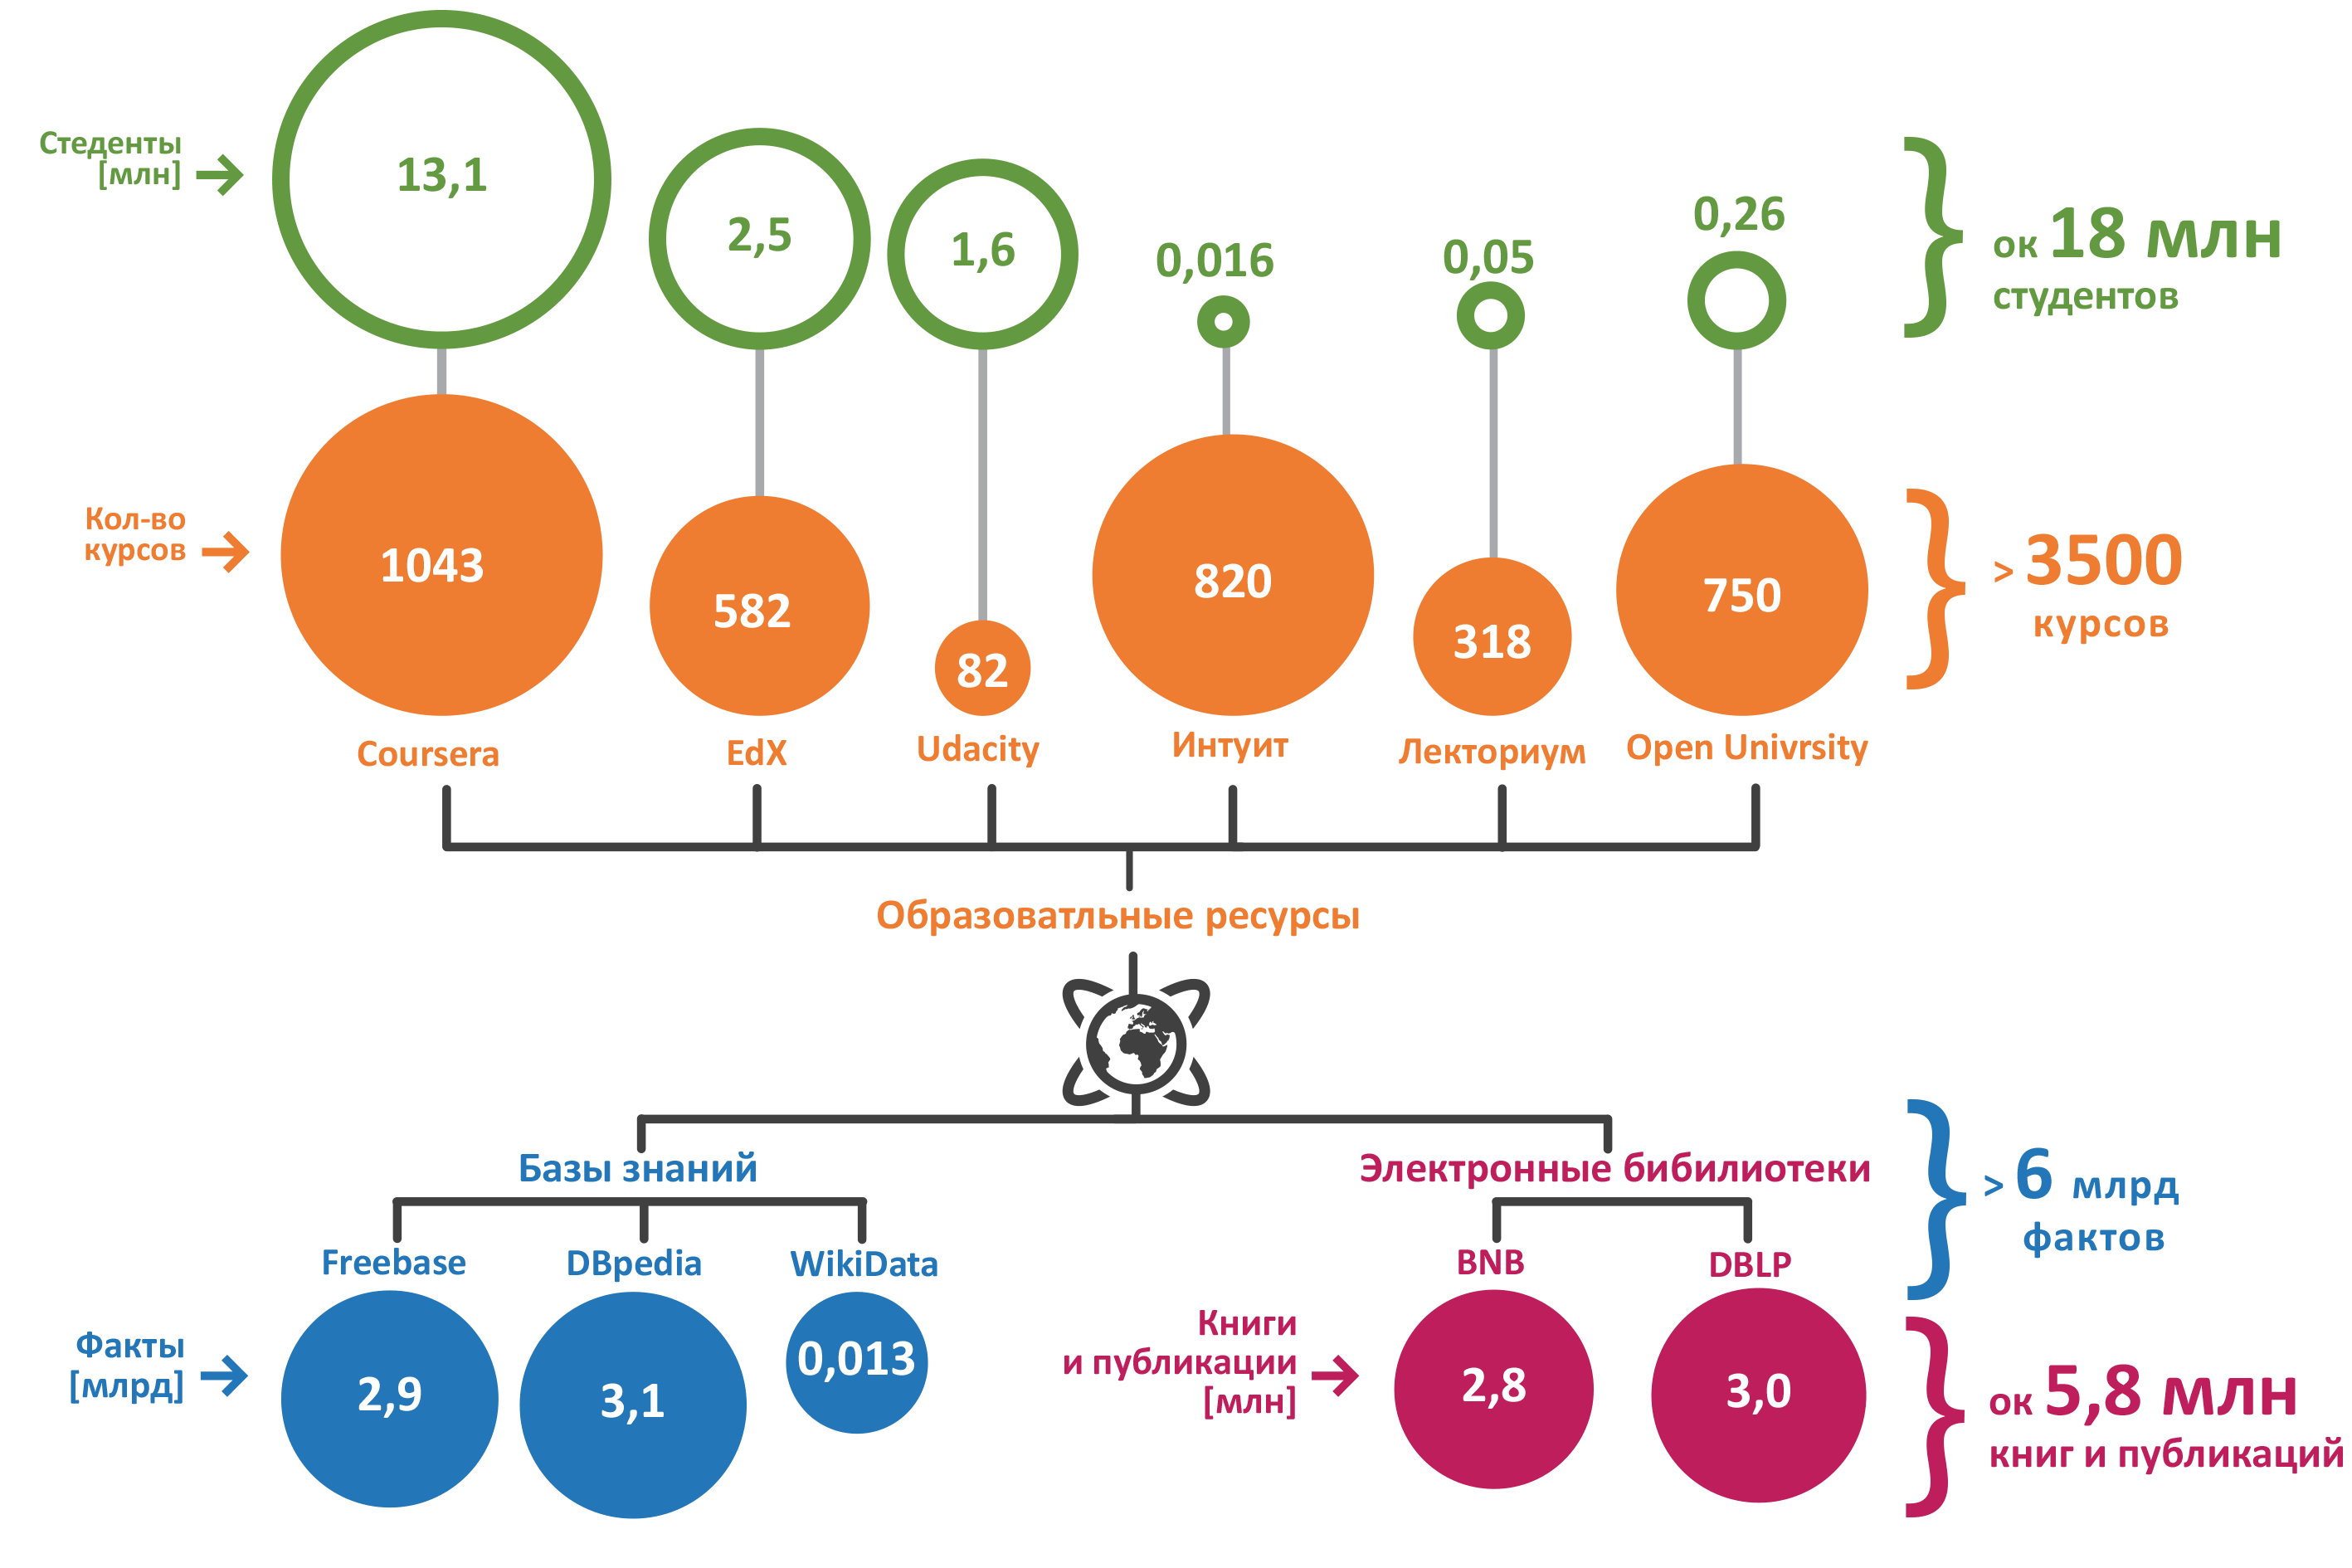
\includegraphics [scale=0.5] {anl_edu_stats}
  \caption{Сводная статистика по образовательным ресурсам, библиотекам и базам знаний.} 
  \label{img:anl_edu_stats}  
\end{figure}


В данный момент существует множество образовательных проектов так или иначе использующих онтологии, технологии Semantic Web и Linked Data. Одним из таких проектов является проект Metacademy. Данный проект представляет собой платформу для открытого  персонализированного образования. В основе обучения в данной системе лежат концепты предметных областей. Пользователь может составить курс или дорожную карту на основе концептов, которые он хочет изучить. Все учебные материалы в системе храняться в онтологиях, что позволяет пользователям производить нелинейную навигацию по теоритическим материалам. В Metacademy весь учебный маетриал, курсы, лекции, книги связаны друг с другом с помощью концептов предметной области.

Другим образовательным проектом использующим семантические технологии является проект SlideWiki \cite{khalili2012slidewiki}. SlideWiki является платформой для создания презентаций для учебных курсов. С помощью семантических технологий платформа позволяет повторно использовать уже опубликованные слайды презентаций, аннатировать дополнительной информацией концепты на слайдах и поддерживать множество языков для одного учебного курса \cite{tarasowa2014crowd}.

Персонализированная образовательная система, основанная на Semantic Web, также обладает сильным аналитическим потенциалом.  Собирая статистические данные по деятельности пользователей в системе, аналитические модули позволяют оценить качество курса, тестов и лекций \cite{aroyo2004new}. Данная статистика получается путем рецензирования пользователями учебных материалов, их посещаемости и популярности. Аналитические механизмы позволяют производить анализ качества учебных курсов и на внутрисистемном уровне, предоставляя преподавателям информацию о степени актуальности модулей курса и степени покрытия курса тестами \cite{puustjarvi2004integrating}.


%%%%%%%%%%%%%%%%%%%%%%%%%%%%%%%%%%%%%%%%%%%%%%%%
% Написать коротко что связи могут использоваться для оценки качества + проблематика
%%%%%%%%%%%%%%%%%%%%%%%%%%%%%%%%%%%%%%%%%%%%

Помимо основной функции системы электронного обучения – образовательного процесса  пользователя системы через взаимодействие с преподавателем и учебным материалом существуют другие направления в дистанционном образовательном процессе, в которых использования технологий Linked Data и Semantic Web предоставляют ряд преимуществ. При организации взаимодействия между пользователями Semantic Web позволяет рядовым пользователям обмениваться и публиковать свои учебные материалы. Онтологические модели позволяют организовывать не только образовательный процесс, но и исследовательский процесс на базе единой системы электронного обучения. Связывания данных направлений реализуется с помощью публикации данных по принципам Linked Data \cite{white2013conceptual}. 


Одним из новых тредов в образовании в России являеться компетентностный подход.
Основная цель профессионального образования – подготовка квалифицированного специалиста соответствующего уровня и профиля, конкурентоспособного на рынке труда, компетентного, свободно владеющего своей профессией и ориентирующегося в смежных областях деятельности, готового к постоянному профессиональному росту, социальной и профессиональной мобильности \cite{chel2013control}. Компетентностный подход не приравнивается к знаниево-ориентированному компоненту, а предполагает целостный опыт решения жизненных проблем, выполнения профессиональных и ключевых функций, социальных ролей, компетенций. При данном подходе в системе электронного обучения оцениваются ключевые компетенции обучаемого отвечающие за его знания, способность к самообразованию, социальные и личностные качества. Для оценки ключевых компетенций система электронного обучения должна интегрировать и анализировать статистические данные связанные не только с проверкой знаний студентов, но и с их взаимодействием с учебными материалами и другими пользователями системы. Семантические технологии позволяют агрегировать данные из социальных что позволяет анализировать социальные и личностные качества обучаемого \cite{abel2013cross}.  

Развитие образовательных систем не стоит на месте и развивается вместе с развитием технологий других отраслей. Образовательный процесс постепенно переходит из университетских аудиторий в виртуальное пространство. Развитие технологи коммуникаций позволяет организовывать виртуальные лекции и конференции. Студенты слушают лекции и проходят стажировки в компаниях, не выходя из дома \cite{masie2012connecting}. Рост количества мобильных устройств среди студентов позволяет им получать учебные материалы, где бы они не находились. Университетские и государственные библиотеки постепенно размещают цифровые копии своих материалов в сети. Пользовательская аудитория систем электронного обучения состоит не только из студентов университетов, но и пользователей с высшим образованием желающих расширить свои знания в той или иной области \cite{oblinger2010campus}. 

Данные факты определяют необходимость тесного взаимодействия информационных технологий и процесса образования. Современная система электронного обучения должна быть ориентирована не только на учащихся определенного университета, а предоставлять учебные курсы всем желающим. Пользователь, не привязанный к определенному университету должен иметь возможность выбора интересующего его направления обучения. 

Поддержка системы электронного обучения крупного масштаба, рассчитанной на большое количество пользователей, не относящихся к какому-либо университету, требует огромных ресурсов. Главными проблемами данной системы являются: 

\begin{itemize}
\item наполнение системы курсам и учебными материалами,
\item поддержка актуальности учебных материалов, 
\item оценка покрытия практическими заданиями теоретических материалов учебного курса,
\item организация проверки знаний обучаемых.
\end{itemize}

Использование онтологий и технологий Semantic Web и Linked Data в системе электронного обучения позволяет решить данные проблемы. Данный подход автоматизирует большинство процессов, позволяя производить следующие действия с системой:

\begin{itemize}
\item автоматический анализ учебных материалов;
\item агрегация, гармонизация и интеграция учебных материалов внешних источников в систему;
\item автоматическая обработка материалов проверки знаний пользователей с дальнейшей публикацией результатов. 
\end{itemize}

Таким образом, создание открытой системы дистанционного обучения на основе технологий Semantic Web и Linked Data, позволяет предоставить обучающимся более гибкий, структурированный и конкретизированный процесс обучения. 


\clearpage
